%share memory
\subsection{Share Memory}
Im Grafikkater ist Zugriff der globale Speicher langsamer als ändere Speicher.  Wie Beispiele in \cite{cudapg} gezeigt, kann man mehrer mal verwendete Daten zunächst in share Memory schreiben, dann für die entsprechenden Operationen benutzen. In der Multiplikation der Vollmatrize mal Vektor wird jede Vektorelement mehr mal gebraut. Nach Untersuchungen wählen wir 1-Dimensionblock,die 64 beträgt und jede Vektorelement 8 mal gebraucht in einem Block, d.h. in jedem Block 8 zerlegende Vektormultiplikation bearbeitet werden. Aus den Ergebnisse von Fig.\ref{sharememory}.(Vergleich von optimierte Vollmatrixmultiplikation mit C-Implementierung und alte GPU-Implementirung für MxN Vollmatrizen).
\begin{figure}[htbp]
%\centering
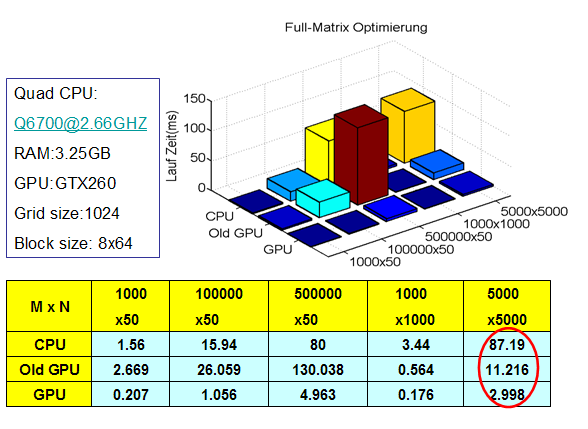
\includegraphics[width=3.5in]{.//pic//sharememory}
\caption{Vergleich von optimierte Vollmatrixmultiplikation mit C-Implementierung und alte GPU-Implementirung für MxN Vollmatrizen}
\label{sharememory} 
\end{figure}

Die optimierte GPU-Implementierung ist immer schnelle als die CPU-Implementierung  und die Alte. Für Matrize 5000x5000 kann die CUDA-Programm 30 mal schneller als CPU
 
